\section{Patterns}
\subsection{Callbacks}
Der Code wird asynchron informiert, wenn sich etwas ändert. Dadurch kann polling verhindert werden, was einen Performance benefit hat. Zudem 
sind die Komponenten besser entkoppelt.
\begin{lstlisting}[language=c]
// Callback type definieren
typedef void (*foo_cbFunction)(int);

// tabelle von pointer fur jedes Event
foo_cbFunction evClient[8] = {0};

// inform
int i = 0;
for (i = 0; i < 8; ++i) {
  if (evClient[i] != 0) {
    evClient[i](arg)	
  }
}
\end{lstlisting}

\subsection{Observer Pattern}
\begin{center}
	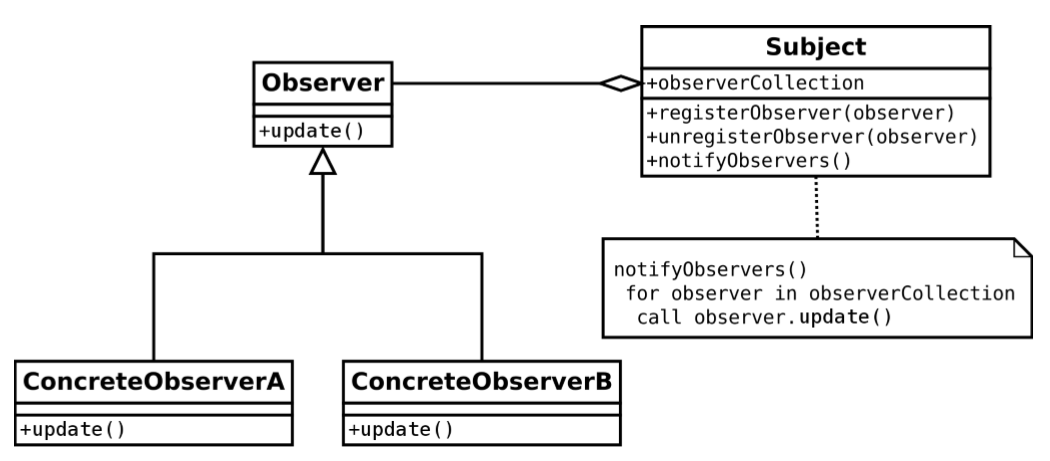
\includegraphics[width=\columnwidth]{Images/observer}
\end{center}
